\documentclass[12pt]{article}
\usepackage{fullpage}
\usepackage{lineno}
\usepackage[notcite,notref]{showkeys}
\usepackage[notcite,notref]{showkeys}
\usepackage{amssymb}
\usepackage{amsmath}
\usepackage{natbib}

\usepackage{epsfig}
\usepackage[mathscr]{eucal}



\bibliographystyle{plain}

%% For lucida bright
%\usepackage[T1]{fontenc}
%\usepackage{lucidabr}
%\usepackage{bm}
%%%




\usepackage{color,amssymb,amsmath,amsthm}

\usepackage{epsfig}
\usepackage[mathscr]{eucal}


\newcommand{\NIW}{near-inertial wave}
\newcommand{\macrot}{macroturbulence}

\newcommand{\com}{\, ,}
\newcommand{\per}{\, .}

%% Averages
% Use \bar to over line solo symbols

\newcommand{\av}[1]{\bar{#1}}
\newcommand{\avbg}[1]{\overline{#1}}
\newcommand{\avbgg}[1]{\overline{#1}}

% A nice definition
\newcommand{\defn}{\ensuremath{\stackrel{\mathrm{def}}{=}}}

% space in equations
\newcommand{\qqand}{\qquad \text{and} \qquad}
\newcommand{\qand}{\quad \text{and} \quad}

% equations
\def\beq{\begin{equation}}
\def\eeq{\end{equation}}

\def\bea{\begin{align}}
\def\ena{\end{align}}


% calculus
\newcommand{\ord}{\mathcal{O}}
%\newcommand{\p}{\partial}
\newcommand{\ii}{{\rm i}}
\newcommand{\dd}{{\rm d}}
\newcommand{\id}{{\, \rm d}}
\newcommand{\ee}{{\rm e}}
\newcommand{\DD}{{\rm D}}
\newcommand{\wavy}{\text{wavy}}
\newcommand{\qg}{\text{qg}}
\newcommand{\dt}{\Delta t}
\newcommand{\dx}{\Delta x}
\newcommand{\be}{\beta}

\newcommand{\al}{\alpha}
\newcommand{\bx}{\boldsymbol{x}}
\newcommand{\by}{\boldsymbol{y}}
\newcommand{\bu}{\boldsymbol{u}}
\newcommand{\bv}{\boldsymbol{v}}


\newcommand{\half}{\tfrac{1}{2}}
\newcommand{\halfi}{\tfrac{\ii}{2}}
\newcommand{\quarter}{\tfrac{1}{4}}
\newcommand{\quarteri}{\tfrac{\ii}{4}}
\newcommand{\halfrho}{\tfrac{1}{2}}
\newcommand{\rz}{{}}
\newcommand{\bn}{\boldsymbol{\hat n}}
\newcommand{\br}{\boldsymbol{r}}
\newcommand{\bR}{\boldsymbol{R}}
\newcommand{\bA}{\ensuremath {\boldsymbol {A}}}
\newcommand{\bB}{\ensuremath {\boldsymbol {B}}}
\newcommand{\bU}{\ensuremath {\boldsymbol {U}}}
\newcommand{\bE}{\ensuremath {\boldsymbol {E}}}
\newcommand{\bN}{\ensuremath {\boldsymbol {\mathrm{N}}}}
\newcommand{\bJ}{\ensuremath {\boldsymbol {J}}}
\newcommand{\bXX}{\ensuremath {\boldsymbol {\mathcal{X}}}}
\newcommand{\bFF}{\ensuremath {\boldsymbol {F}}}
\newcommand{\bF}{\ensuremath {\boldsymbol {F}^{\sharp}}}
\newcommand{\bG}{\ensuremath {\boldsymbol G}}
\newcommand{\bSigma}{\ensuremath {\boldsymbol {\Sigma}}}
\newcommand{\bvarphi}{\ensuremath {\boldsymbol {\varphi}}}
\newcommand{\bxi}{\ensuremath {\boldsymbol {\xi}}}
\newcommand{\avbxi}{\overline{\ensuremath {\boldsymbol {\xi}}}}

% math cal

\newcommand{\J}{\mathcal{J}}
\newcommand{\K}{\mathcal{K}}
\newcommand{\cG}{\mathcal{G}}
\newcommand{\cF}{\mathcal{F}}
\newcommand{\cN}{\mathcal{N}}
\newcommand{\cL}{\mathcal{L}}
\newcommand{\cS}{\mathcal{S}}
\newcommand{\cE}{\mathcal{E}}


% san serif for matrices and differential operators
%\newcommand{\helmn}{\mathsf{H}_n}
\newcommand{\helmm}{\triangle_m}
\newcommand{\helmn}{\triangle_n}
\newcommand{\helms}{\triangle_s}
\newcommand{\helm}{\triangle}
\newcommand{\sA}{\mathsf{A}}
\newcommand{\sB}{\mathsf{B}}
\newcommand{\sG}{\mathsf{G}}
\newcommand{\sI}{\mathsf{I}}
%\newcommand{\sJ}{\mathsf{J}}
\newcommand{\sJ}{J}
\newcommand{\gsJ}{\breve{\mathsf{J}}}
\newcommand{\sU}{\mathsf{U}}
\newcommand{\sP}{\mathsf{P}}
\newcommand{\sQ}{\mathsf{Q}}
\newcommand{\sR}{\mathsf{R}}
\newcommand{\sL}{\mathsf{L}}
\newcommand{\Lu}{\mathsf{L}(\what{u}_k)}
\newcommand{\Nu}{\mathsf{N}(\what{u}_k)}
\renewcommand{\L}{\mathsf{L}}
\newcommand{\N}{\mathsf{N}}
\newcommand{\sH}{\mathsf{H}}
\renewcommand{\sI}{\mathsf{I}}
\renewcommand{\L}{\mathsf{L}}
\newcommand{\sM}{\mathsf{M}}
\newcommand{\sT}{\mathsf{T}}
\newcommand{\sGamma}{\mathsf{\Gamma}}
\newcommand{\sOmega}{\mathsf{\Omega}}
\newcommand{\sSigma}{\mathsf{\Omega}}
\newcommand{\sbeta}{\mathsf{\beta}}
\newcommand{\sPi}{\mathsf{\Pi}}
\newcommand{\sC}{\mathsf{C}}
\newcommand{\sQy}{\mathsf{Q}}
\renewcommand{\sb}{\mathsf{b}}

% u
\newcommand{\uhat}{\what{u}_k}

% angle brackets

\def\la{\langle}
\def\ra{\rangle}
\def\laa{\left \langle}
\def\raa{\right \rangle}


%grads and div's
%\newcommand{\bcdot}{\hspace{-0.1em} \boldsymbol{\cdot} \hspace{-0.12em}}
%\newcommand{\bnabla}{\boldsymbol{\nabla}}
\newcommand{\bnablaH}{\bnabla_{\! \mathrm{h}}}
\newcommand{\grad}{\bnabla}
\newcommand{\gradH}{\bnablaH}
\newcommand{\curl}{\bnabla \!\times\!}
\newcommand{\diver}{\bnabla \! \bcdot \! }
\newcommand{\cross}{\times}
%\newcommand{\lap}{\nabla^2}
\newcommand{\lap}{\triangle}

%varthetas and thetas
\newcommand{\vth}{\vartheta}
\newcommand{\psii}{\psi^{\mathrm{i}}}
\newcommand{\thb}{\theta^{\mathrm{-}}}
\newcommand{\vthb}{\vartheta^{\mathrm{-}}}
\newcommand{\vthbhat}{{\hat{\vartheta}}^{\mathrm{-}}}
\newcommand{\vThb}{\varTheta^{\mathrm{-}}}
\newcommand{\psib}{\psi^{\mathrm{-}}}
\newcommand{\tht}{\theta^{\mathrm{+}}}
\newcommand{\vtht}{\vartheta^{\mathrm{+}}}
\newcommand{\vththat}{{\hat{\vartheta}}^{\mathrm{+}}}
\newcommand{\vthtbhat}{{\hat{\vartheta}}^{\pm}}
\newcommand{\vTht}{\varTheta^{\mathrm{+}}}
\newcommand{\vthtb}{\vartheta^{\pm}}
\newcommand{\vThtb}{\varTheta^{\pm}}

% nondimensional numbers
\renewcommand{\Re}{\mathrm{Re}}
\newcommand{\Ro}{\mathrm{Ro}}
\newcommand{\Bu}{\mathrm{Bu}}
\newcommand{\Ri}{\mathrm{Ri}}

%psi's
%Galerking coefficient for psi:
\newcommand{\gpsi}{\breve \psi}
\newcommand{\gpsic}{{\breve \psi}^\star}
\newcommand{\gtau}{\breve \tau}
\newcommand{\gtauc}{{\breve \tau}^\star}
\newcommand{\gphi}{\breve \phi}
\newcommand{\gq}{\breve q}
\newcommand{\gU}{\breve U}
\newcommand{\gQ}{\breve Q}
\newcommand{\gsigma}{\breve \sigma}


\newcommand{\psit}{\psi^{\mathrm{+}}}
\newcommand{\psithat}{{\hat{\psi}}^{\mathrm{+}}}
\newcommand{\psibhat}{{\hat{\psi}}^{\mathrm{-}}}
\newcommand{\psitb}{\psi^{\pm}}
\newcommand{\psitbhat}{{\hat{\psi}}^\pm}
\newcommand{\St}{S^{\mathrm{+}}}
\newcommand{\Sb}{S^{\mathrm{-}}}
\newcommand{\phb}{\phi^{\mathrm{-}}}
\newcommand{\pht}{\phi^{\mathrm{+}}}
\newcommand{\tautb}{\tau^{\pm}}
\newcommand{\sigmatb}{\sigma^{\pm}}


\newcommand{\bur}{\left(\tfrac{f_0}{N}\right)^2}
\newcommand{\ibur}{\left(\tfrac{N}{f_0}\right)^2}
\newcommand{\Nm}{N_{\mathrm{mix}}}
\newcommand{\xim}{\xi_{\mathrm{mix}}}
\newcommand{\hs}{h_*}
\renewcommand{\sp}{\mathsf{p}}
\newcommand{\se}{\mathsf{e}}
\newcommand{\sptb}{\mathsf{p}^\pm}


%nmax is a problem:
%\newcommand{\nmax}{n_{\mathrm{max}}}
\newcommand{\nmax}{\mathrm{N}}
\newcommand{\mmax}{\mathrm{M}}

\newcommand{\WKB}{\mathrm{WKB}}
\newcommand{\Lam}{\Lambda}
\newcommand{\tha}{\theta}
\newcommand{\kap}{\kappa}
\newcommand{\bphi}{\boldsymbol{\phi}}
\newcommand{\third}{\tfrac{1}{3}}
\newcommand{\cs}{c^\star}
\newcommand{\dstar}{{\star\star}}
\newcommand{\nt}{n^{\mathrm{trnc}}}
\newcommand{\sDp}{\mathsf{D}^1_{\nmax}}
\newcommand{\sDpp}{\mathsf{D}^2_{\nmax}}
\newcommand{\sD}{\mathsf{D}}
\newcommand{\sDN}{\mathsf{D_\nmax}}
\newcommand{\sK}{\mathsf{K_2}}
\newcommand{\stheta}{\mathsf{\theta}}
\newcommand{\sphi}{\mathsf{\phi}}
\newcommand{\sq}{\mathsf{q}}
\newcommand{\cosech}{\text{csch}\,}
\newcommand{\sinc}{\text{sinc}\,}

%%%%%%%%% %%%%

%%%%%%%%% %%%%
\newcommand{\zt}{z^+}
\newcommand{\zb}{z^-}
\newcommand{\qA}{q^A_{\nmax}}
\newcommand{\psiB}{\psi^B_{\nmax}}
\newcommand{\phiB}{\phi^B_{\nmax}}
\newcommand{\eye}{\boldsymbol{\hat{i}}}
\newcommand{\jay}{\boldsymbol{\hat{j}}}
\newcommand{\kay}{\boldsymbol{\hat{k}}}
\newcommand{\psiG}{\psi^{\mathrm{G}}}
\newcommand{\qG}{q^{\mathrm{G}}}
\newcommand{\uG}{u^{\mathrm{G}}}
\newcommand{\UG}{U^{\mathrm{G}}}
\newcommand{\UGN}{U^{\mathrm{G}}_{\nmax}}
\newcommand{\QGN}{Q^{\mathrm{G}}_{\nmax}}
\newcommand{\sumoddn}{\sum_{n = 1, n~ \text{odd}}^{\nmax}}

% bretherton
\newcommand{\qBr}{q_{\mathrm{Br}}}
\newcommand{\psiBr}{\psi_{\mathrm{Br}}}

\newcommand{\ep}{\epsilon}
\newcommand{\vep}{\varepsilon}


%\renewcommand{\sZ}{\mathsf{Z}}
%\renewcommand{\sE}{\mathsf{E}}
%\newcommand{\iBu}{\left(\tfrac{f_0}{N}\right)^2}
\newcommand{\F}{\mathcal{F}}
\newcommand{\D}{\mathcal{D}}
\newcommand{\phis}{\phi^\star}

%\newcommand{\bk}{\boldsymbol{k}}

\newcommand{\cg}{\mathbf{c}_g}
\newcommand{\Uf}{\mathbf{U}}
\renewcommand{\Im}{\mathrm{Im}}
\renewcommand{\div}{\nabla\cdot}
\renewcommand{\P}{\mathcal{P}}
\newcommand{\dU}{\delta U}
\newcommand{\W}{\mathcal{W}}
\newcommand{\cK}{\mathcal{K}}
\newcommand{\cP}{\mathcal{P}}
\renewcommand{\L}{\mathsf{L}}
\renewcommand{\N}{\mathsf{N}}
\newcommand{\psiq}{\psi^q}
\newcommand{\psiw}{\psi^w}
%\newcommand{\tfrac}{\frac}
%\newcommand{\eqref}{\ref}
\newcommand{\kb}{\mathbf{k}}
\newcommand{\xb}{\mathbf{x}}
%wave PV
\newcommand{\qw}{q^{\mathrm{w}}}
\newcommand{\bw}{b^{\mathrm{w}}}
\newcommand{\ug}{u^{\mathrm{g}}}
\newcommand{\bug}{\bu^{\mathrm{g}}}

%action and energy
\newcommand{\Ewn}{E}
\newcommand{\A}{  \mathcal{A}}
\newcommand{\E}{\mathcal{E}}
\newcommand{\Pw}{\mathcal{P}}
\newcommand{\Ke}{\mathcal{K}}
\newcommand{\Ff}{ \boldsymbol{\mathcal{F}}}
\newcommand{\Ffp}{\boldsymbol{\mathcal{F}}^{\perp}}
\newcommand{\Hf}{\boldsymbol{\mathcal{H}}}
\newcommand{\Gg}{\boldsymbol{\mathcal{G}}}
\newcommand{\epA}{\varepsilon_\mathcal{A}}
\newcommand{\epP}{\varepsilon_\mathcal{P}}
\newcommand{\epK}{\varepsilon_\mathcal{K}}

%dispersivity
\newcommand{\disp}{\eta}

%relative vorticity
\newcommand{\ze}{\zeta}

% index differentiation
\newcommand{\gind}[2]{#1_{,#2}}

% QG-NIW model (or XV model)
\newcommand{\coupledmodel}{QG-NIW model}

% expectation
\newcommand{\Es}{\mathbb{E}}

% math
\newcommand{\p}{\partial}
\newcommand{\bcdot}{\hspace{-0.1em} \boldsymbol{\cdot} \hspace{-0.12em}}
\newcommand{\bnabla}{\boldsymbol{\nabla}}

\begin{document}


\title{Equilibration of forced barotropic turbulence by stimulated generation
of near-inertial waves}

\author{
CR  \& WRY \thanks {Scripps Institution of Oceanography,
University of California at San Diego, La Jolla, CA
92093--0230, USA.
%\protect\url{email:wryoung@ucsd.edu}.
}
}


\maketitle

\section{The model}

In the vertical plane-wave model, waves affect the balanced
flow via rectification terms in the quasi-geostrophic potential vorticity $q$:
\beq
\label{qgpv}
q = \underbrace{\lap \psi}_{\defn \zeta} +
                \underbrace{\tfrac{1}{f_0}\Big[ \tfrac{1}{4} \lap |\phi|^2 + \tfrac{\ii}{2}
                \sJ(\phi^\star,\phi)\Big]}_{\defn q^w}\com
\eeq
where $\psi(x,y,t)$ is the wave-averaged streamfunction and $\phi(x,y,t)$ is the near-inertial
back-rotated velocity of a vertical plane wave with wavenumber m; the total
horizontal velocity is
\beq
\label{phi}
u + \ii v =  \phi \ee^{\ii\varpi}-\psi_y + \ii \psi_x\com
\eeq
where $\varpi \defn m z -f_0 t$ is the phase of the near-inertial wave.

%\newcommand{\F}{\mathcal{F}}
\subsection{The forced potential vorticity equation: balanced dynamics}
The balanced dynamics satisfy the potential vorticity equation
\beq
q_t + \sJ(\psi,q)  = \F_q -\mu \zeta + \D_q \com
\label{balanced_dynamics}
\eeq
where $\mu$ is the linear bottom drag. And $\F_q$ is a
stochastic forcing that renovates every $\tau$,
\renewcommand{\Hf}{\mathcal{H}}
\beq
\label{F_q}
\F_q = \xi_q(x,y,t)/\tau^{1/2}\com
\eeq
where $\xi_q$ is a normally-distributed random field with annular horizontal wavenumber spectrum
centered at $k_f$:
\beq
\label{spec_forcing}
\Es(\hat{\xi_q^\star}\hat{\xi_q}) =  A \exp\big\{{-[(k^2+l^2)^{1/2}-k_f]^2/2\Delta_f^2}\big\};
\eeq
$\Delta_f$ is the width of the spectrum; and $\hat{\xi_q}$ is the Fourier transform of $\xi_q$:
\beq
\hat{\xi_q}(k,l) = \frac{1}{(2\pi)^2}\iint \xi_q(x,y)\ee^{\ii(kx + ly)}\dd k \dd l\per
\eeq
The constant A is determined by the normalization condition,
\beq
\label{norm_fq}
\frac{1}{(2\pi)^2}\iint\half(k^2 + l^2)^{-1}\Es(\hat{\xi_q^\star}\hat{\xi_q}) \dd k \dd l= \sigma_q^2\per
\eeq

In the waveless case, this normalization ensures that
the expectation of the energy input equals the variance of the forcing $\sigma_q^2$:
\beq
\Es[\xi_q(n)\xi_q(m)]= \sigma_q^2 \tau \delta_{mn}\,;
\eeq
see discussion in the next section.

The white-noise forcing requires a renovation time scale smaller than
the numerical time step, $\tau \ll \Delta t$. For numerical implementation,
however, we are forced choose $\tau = \Delta t$. The stochastic forcing $\F_q$
is thus only an approximation to white noise. The white-noise approximation is
accurature provided $\Delta t \ll (k_f U)^{-1}$, where $U$ is the root-mean-square
velocity of the turbulence. This requirements is satisfied in all solutions discussed
below. We thus loosely refer to $\F_q$, and
the wave forcing $\F_\phi$ defined below, as white-noise throughout.


%  And the horizontal structure of the forcing, $\Hf(x,y)$, also renovates every the wavenumber spectrum of the forcing is
\subsection{The vertical plane-wave YBJ equation: wave dynamics}
The vertical plane-wave model is completed by the YBJ equation for the evolution
of the back-rotated near-inertial velocity $\phi$:
\beq
\phi_t + \sJ(\psi,\phi) +  \phi \tfrac{\ii}{2}\ze - \tfrac{\ii}{2} \disp \lap \phi
 = \F_\phi -\gamma \phi + \D_\phi\com
 \label{ybj_dynamics}
\eeq
$\eta = f_0\lambda^2$ is the wave dispersivity and  $\gamma$
is a linear damping coefficient, which is related to the vertical viscosity
that damps the near-inertial velocity:
\beq
\nu \p_z^2(\phi \ee^{\ii \varpi}) = - \underbrace{m^2\nu}_{\defn \gamma}\phi\com
\eeq
where $\varpi = mz - f_0 t$. Vertical viscosity parameterizes
all processes---including wave-wave interactions---that were neglected by the
asymptotic derivation of \eqref{ybj_dynamics}.

Also in \eqref{ybj_dynamics}, $\F_\phi(t)$ is a stochastic forcing that renovates
every $\tau$ with variance $\Es(\F_\phis\F_\phi) = \sigma_\phi^2$; $\F_\phi$ has
no spatial structure. The advantage of forcing the waves with this type of stochastic
forcing is that the rate of energy input by the forcing is predicted. We experimented
with constant and shot-noise forcings. The results from these experiments are
 qualitatively similar results to the solutions forced by white-noise.

In \eqref{balanced_dynamics} and \eqref{ybj_dynamics}, $\D_q$ and $\D_{\phi}$ represent
small-scale horizontal dissipation, which are necessary for numerical stability.
In practice, we use an exponential spectral filter, which selectively damps aliased
wavenumbers. In the solution described bellow, small-scale horizontal dissipation contributes
insignificant sinks to the energy budgets.

% Talk about forcing as an approximation to white-noise.

\subsection{Power integrals}

The wave action equation is
\beq
\frac{\dd}{\dd t} \underbrace{\tfrac{1}{2 f_0} \la |\phi|^2 \ra}_{\defn \A} = \tfrac{1}{2f_0}\la \phis \xi_\phi +
\phi \xi_\phis \ra -\tfrac{1}{f_0}\gamma \la |\phi|^2 \ra + \tfrac{1}{2f_0} \la \phis\D_\phi + \phi\D_\phis \ra\com
\label{A}
\eeq
where $\la\,\ra$ represents spatial average. In the white-noise limit, the expectation for
the work due the wave forcing is
\beq
\Es\Big(\tfrac{1}{2}\la \phis \xi_\phi+\phi \xi_\phis \ra\Big) = \half\sigma_\phi^2\per
\eeq
And we obtain a prediction for the equilibrated wave action:
\beq
\label{prediced_A}
\Es(\A) = \frac{\sigma_\phi^2}{2 f_0 \gamma}\com
\eeq
provided that small-scale dissipation $\tfrac{1}{2f_0}\la\phis\D_\phi+\phi\D_\phis\ra$
is insiginificant.

The balanced kinetic energy equation is
\beq
\frac{\dd}{\dd t} \underbrace{\half \la |\nabla \psi|^2 \ra}_{\defn \K} = -(\Gamma_r + \Gamma_a) + \Xi
 -\la \psi \F_q \ra -\ \mu \la|\nabla\psi|^2\ra - \la\psi\D_q\ra\per
\label{Ke}
\eeq
Above, $\Gamma_r$ and
$\Gamma_a$ are energy conversion terms,
\begin{align}
\Gamma_r &\defn  \Big\la\half\ze \, \diver\Ff \Big\ra\com \label{convr}
\end{align}
where the wave action flux is
\beq
\label{Fw2}
\Ff \defn \tfrac{\ii}{4}\lambda^2 \left(\phi\grad\phis-\phis\grad\phi\right);
\eeq
and
\beq
 \Gamma_a \defn -\tfrac{\lambda^2}{2}
   \left\la
   \begin{bmatrix}
   \phi_x^\star & \phi_y^\star
   \end{bmatrix}
   \begin{bmatrix}
   -\psi_{xy} & \half(\psi_{xx} - \psi_{yy})\\
   \half(\psi_{xx}-\psi_{yy}) & \psi_{xy}
\end{bmatrix}
 \begin{bmatrix}
   \phi_x \\  \phi_y
   \end{bmatrix}\right\ra\per
   \label{conva}
\eeq
 Also in \eqref{Ke}, $\Xi$ is a source of balanced kinetic energy
due to wave dissipation:
\beq
\label{Xi}
\Xi = -\gamma\left[\left\la\A \half\zeta\right\ra +
        \eta^{-1}\la\mathbf{u}_g\bcdot\Ff\ra\right]
    + \half f_0^{-1}\left[\left\la (\phis\D_\phi+\phi\D_\phis)\half\zeta\right\ra\right]
      + \mathbf{u}_q\bcdot\halfi (\D_\phi\grad\phis-\D_\phis\grad\phi)\com
\eeq
where $\mathbf{u}_g = \hat{\mathbf{z}}\cross\grad\psi$ is the geostrophic velocity;
$\Xi$ is a form of ``wave streaming.''
The first two terms in \eqref{Xi} stem from linear dissipation of $\phi$. The first
terms shows that the dissipation of wave action in anticylones is a source of balanced
kinetic energy. The second term shows that the alignment of the geostrophic velocity
with the wave action density flux is a sink of balanced kinetic energy. The
remanining two terms stem from small-scale dissipation.
See \cite{rocha_etal2017} for a derivation of $\Gamma_r$, $\Gamma_a$, and $\Xi$.

In the waveless case, $\phi(t=0)=0$ and $\F_\phi=0$,  which implies that
$\Gamma_r=\Gamma_a = \Xi = 0$. In the white-noise limit, the waveless expectation for
the work delivered by the forcing is
\beq
\Es\big(-\la\psi\xi_q\ra\big) = \sigma_q^2\per
\eeq
We thus obtain a prediction for the equilibrated balanced kinetic energy in the
absence of waves:
\beq
\label{predicted_K}
\Es(\K )= \frac{\sigma_q^2}{\mu}\com
\eeq
provided that small-scale dissipation $-\la\psi\D_q\ra$ is insignificant.

Finally, the potential energy equation  is
\beq
\frac{\dd}{\dd t} \underbrace{\tfrac{\lambda^2}{4} \la |\nabla\phi|^2 \ra}_{\defn \P} = \Gamma_r + \Gamma_a
 -\tfrac{\lambda^2}{2}\gamma \la |\nabla\phi|^2 \ra - \tfrac{\lambda^2}{2} \la \lap\phis\D_\phi + \lap\phi\D_\phis \ra\per
\label{P}
\eeq
Note that there's no external generation of wave potential energy $\P$ because the
stochastic forcing has no spatial scale. $\P$ is only created by stimulated generation represented
by the conversion terms $\Gamma_r$ and $\Gamma_a$. In statistical steady state, the
wave potential energy created by stimilated generation dissipates via $-2\gamma\P$,
 provided there's insignificant small-scale dissipation. But this isn't a prediction
 for $\P$ since $\Gamma_a$ and $\Gamma_r$ are functions of $\phi$.

\section{A reference solution}

\begin{table}
 \begin{center}
   \caption{Details of the reference solution.}
   \label{parameters_reference}
   \begin{tabular}{ l | l | l }
     \hline
      Parameter & Description & Value \\
      \hline
      $\mathsf{N}$   & Number of modes &  512  \\
      $L_d$ & Domain size & $2\pi\times 200$ km \\
      $\sigma_q^2$ & Balanced-forcing variance & $1.45\,\,10^{-8}$ m$^2$ s$^{-3}$ \\
      $\sigma_w^2$ & Wave-forcing variance & $5.78\,\,10^{-8}$ m$^2$ s$^{-3}$ \\
      $k_f L_d/2\pi$    & Balanced-forcing wavenumber & 8 \\
      ${dk}_f L_d/2\pi$    & Balanced-forcing width &  1 \\
      $\mu$ & Linear bottom drag coefficient & $5.78\,\,10^{-8}$ s$^{-1}$ \\
      $\gamma$ & Linear wave damping coefficient & $2.31\,\,10^{-7}$ s$^{-1}$ \\
      $N$ & Buoyancy frequency &  $5\,\,10^{-3}$ s$^{-1}$\\
      $f_0$ & Coriolis frequency &  $1\,\,10^{-4}$ s$^{-1}$\\
      $\D_\phi$ & Exponential spectral filter & ---\\
      $\D_q$ & Exponential spectral filter & ---\\
   \end{tabular}
 \end{center}
\end{table}

\begin{figure}
\centering
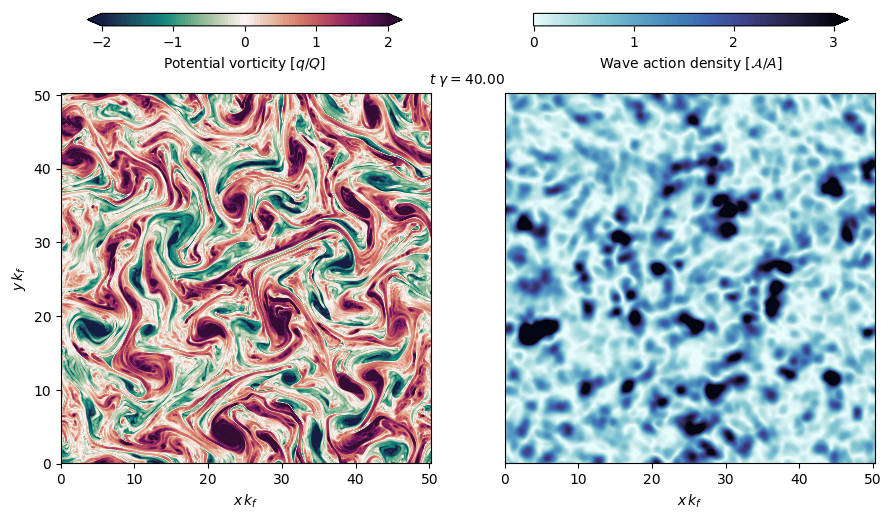
\includegraphics[width=.925\textwidth]{figs/snapshots_pv_qg-niw_reference.png}
\caption{Snapshot of potential vorticity and wave action density for the solution
         with parameters in  table \ref{parameters_reference}. The scale of potential vorticity
         is $Q = \sigma_q/\mu^{1/2} $ and the scale of wave action density is
         $A = \sigma_w^2/f_0 \gamma$.}
        \label{snapshots_pv_qg-niw_reference}
\end{figure}

Figure \ref{snapshots_pv_qg-niw_reference} shows snapshots of potential vorticity and wave
action density for a solution with $\sigma_w^2 = 2\sigma_q^2$ and $\gamma = 4\mu$; table
\ref{parameters_reference} describes in detail the parameters of
this reference solution. The equilibrated potential vorticity in figure
\ref{snapshots_pv_qg-niw_reference}a  resembles the vorticity field
of waveless two-dimensional turbulence with its ubiquitous eddies, filaments,
and coherent structures. A main difference is that the the potential vorticity
of this wave-modified turbulence is more fine-grained (see spectrum?).

The snapshot of wave action density depicts the incoherent nature of the equilibrated
wave field, which is being scrambled by the turbulent balanced field
(figure \ref{snapshots_pv_qg-niw_reference}b). The wave field develops scales smaller
than the balanced eddies due to straining by the flow and wave interference.
The snapshot in \ref{snapshots_pv_qg-niw_reference}b resembles the wave field in decaying wave-modified
two-dimensional turbulence (RWY).

Figure \eqref{energies_reference} shows time series of balanced kinetic energy
and wave action and wave potential energy. The system equilibrates after $\sim\!1
\, \mu^{-1} = 4 \gamma^{-1}$. Wave action $\A$ displays large fluctuations ($50\%$ of
 the time-average equilibrated value). Balanced kinetic energy $\K$
and wave potential energy $\P$, on the other hand, show much smaller fluctuations
($10\%$ of the equilibrated levels). Interestingly, $\K$ and $\P$ fluctuate
largely out of phase.

The wave kinetic energy equilibrate at 60\% of theoretical prediction for waveless
turbulence forced by white-noise: $\Es(\K) = \sigma_q^2/\mu$. And the wave potential
energy equilibrates at about $10\%$ of the wave kinetic energy level, which suggests
that stimulated generation plays a crucial role in the equilibration of forced
barotropic turbulence.  Indeed, figure \ref{energy_budgets_reference}a shows that
stimulated generation, $-(\Gamma_r+\Gamma_a)$ in \eqref{Ke}, contributes about half
of the sink of wave kinetic energy---bottom drag,
$-2\mu \K$ in  \eqref{Ke}, accounts for the other half. Wave streaming, $\Xi$ in
\eqref{Ke}, is small but significant: $\Xi$ contributes about 5\% source of $\K$.
See table X1 for details of the budget.

The wave potential energy budget (figure \ref{energy_budgets_reference}b) confirms that
linear dissipation $-2\gamma \P$ damps most of $\P$ created via stimulated generation;
the residual is smaller than $1\%$ (table X2). Similarly, linear dissipation
$-2\gamma \A$ removes virtually all the wave action
$\A$ input by the white-noise forcing. While the forcing input is nearly constant,
wave action and the linear dissipation are highly intermitent. Thus, vertical viscosity damps the waves
and the details of small-scale horizontal dissipation are irrelevant for the energy budget.

The balanced kinetic energy spectrum is shallower at submesoscales compared to
waveless turbulence. Stimulated generation also appears to slow down the
inverse cascade of balanced kinetic energy: there's more energy at large-scales
in the spectrum of waveless turbulence. The wave action has a nearly flat spectrum
between the forcing scale $k_f$ and the dissipative scale $k_d$.

\begin{figure}
\centering
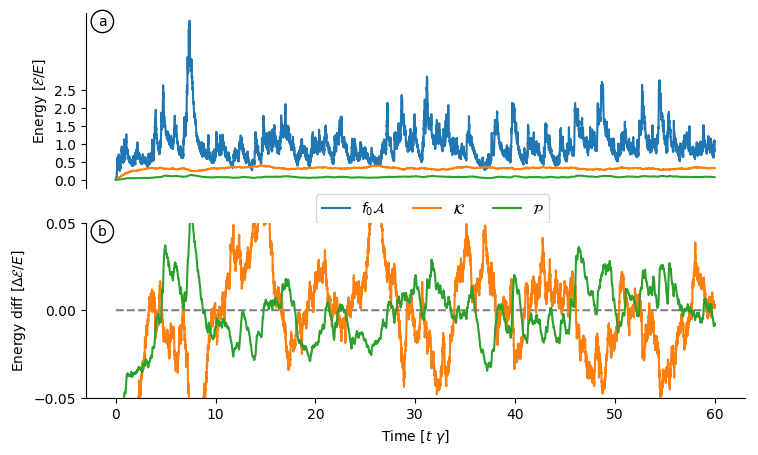
\includegraphics[width=.825\textwidth]{figs/energies_reference.png}
\caption{(a) Balanced kinetic energy ($\K$) and wave potential energy ($\P$) and wave
         kinetic energy ($f_0 \A$)  for the solution with parameters in table
         \ref{parameters_reference}. The energy difference, $\Delta \K$ and $\Delta \P$,
         about a time average after equilibration ($t\,\gamma \ge 5$).}
        \label{energies_reference}
\end{figure}

\begin{figure}
\centering
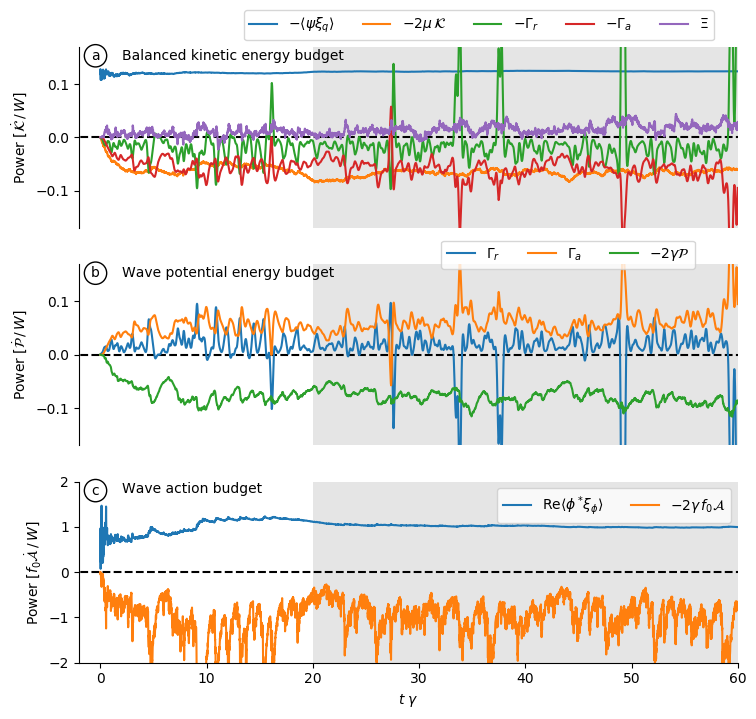
\includegraphics[width=.825\textwidth]{figs/K_and_P_and_A_budget_reference.png}
\caption{The budget of (a) balanced kinetic energy ($\K$), wave potential energy ($\P$),
        and (c) wave
         kinetic energy ($f_0 \A$)  for the solution with parameters in table
         \ref{parameters_reference}. The power is scaled by the work due to the
         wave forcing $W=\sigma_w^2/2$.}
        \label{energy_budgets_reference}
\end{figure}


\begin{figure}
\centering
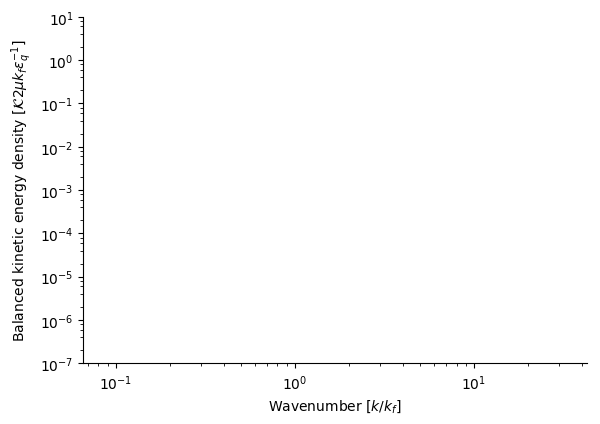
\includegraphics[width=.925\textwidth]{figs/spectrum_qg-niw.png}
\caption{Spectra of balanced kinetic energy (a) and wave kinetic and potential
          energies (b) calculated after equilibration ($t\,\gamma \ge 5$). The
          dashed line in (a) shows the balanced kinetic energy spectrum from a
          reference waveless simulation.}
        \label{spectra_reference}
\end{figure}

\bibliography{ForcedQGNIW.bib}

\end{document}
